\documentclass{beamer}
\DeclareFontShape{OT1}{cmss}{b}{n}{<->ssub * cmss/bx/n}{} 
\usetheme{CambridgeUS}
\usepackage{amsmath}
\usepackage{amsfonts}
\usepackage{mathbbol}
\usepackage{xcolor} % before tikz or tkz-euclide if necessary
\usepackage{tkz-euclide} % no need to load TikZ
\usepackage{multirow}
\usepackage{lmodern}
\usepackage{bm}

\usepackage[
backend=biber,
style=authoryear-icomp,
sortlocale=de_DE,
natbib=true,
url=false, 
doi=true,
eprint=false
]{biblatex}
\addbibresource{../../Bibliography/main_ML.bib}



\titlegraphic{\includegraphics[width=2cm]{../../Figures/UAMS_RGB.png}
}


\title{Statistical Machine Learning\\ Activation Functions}
\author{Horacio G\'omez-Acevedo\\ Department of Biomedical Informatics\\
	University of Arkansas for Medical Sciences}
\begin{document}
	\begin{frame}[plain]
		\maketitle
	\end{frame}

\begin{frame}{What are activation functions?}
Recall that in the threshold logic,  once we receive the input, a decision must be made to \textit{fire} or \textit{suppress} the output. 

\begin{figure}[h]
	\centering
	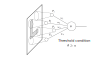
\includegraphics[scale=0.8]{../../Figures/fig_threshold.png}
\end{figure}

\end{frame}
\begin{frame}{Activation functions}
	


\textbf{Activation functions} generalize the concept of activation given a specific  input.

\begin{figure}[h]
	\centering
	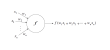
\includegraphics[scale=0.8]{../../Figures/fig_activation.png}
\end{figure}
	
\end{frame}

\begin{frame}{Linear Functions}
	
	These functions are used to model the firing rate of a neuron.
	
	\begin{equation*}
		f(x)= kx \quad k \text{ is a positive constant}
	\end{equation*}

Pros: It is continuous and differentiable.	

\begin{figure}[h]
	\centering
	\includegraphics[scale=0.8]{../../Figures/fig_activation_21.png}
\end{figure}

	
\end{frame}

\begin{frame}{Step Functions}
	These are biologically inspired type of activation.
	
	\begin{enumerate}
		\item Heaviside function (threshold step function). This function fires only for positive values.
		\begin{equation*}
			H(x)=
			\begin{cases}
				0 & \text{if }x\le 0 \\
				1 & \text{if } x >0
			\end{cases}
		\end{equation*}
	
	\end{enumerate}
\begin{figure}[h]
	\centering
	\includegraphics[scale=0.5]{../../Figures/fig_activation_22}
\end{figure}

This function is differentiable except in $x=0$.  Informally, people refers to the Dirac delta function as its \textit{derivative}. 
\begin{equation*}
	H'(x)= \delta(x) =\begin{cases}
		0 & \text{if } x \ne 0,\\
		\infty & \text{if } x=0
	\end{cases} \quad \text{it also satisfies} \int_{-\infty}^{\infty} \delta(x)dx =1
\end{equation*}


\end{frame}



\begin{frame}{Step Functions (cont)}
	\begin{enumerate}
		\setcounter{enumi}{1}
		\item Signum Function. This is a variation of the Heaviside function
		\begin{equation*}
			S(x)= \begin{cases}
				-1 & \text{if } x <0 \\
				1 & \text{if } x \ge 0
			\end{cases}
		\end{equation*}
	\end{enumerate}
\begin{figure}[h]
	\centering
	\includegraphics[scale=0.8]{../../Figures/fig_activation_22b}
\end{figure}
\end{frame}

\begin{frame}{Hockey stick functions}
	\begin{enumerate}
		\item Rectified Linear Unit (ReLu). The activation is linear for $x\ge 0$.
		\begin{equation*}
			ReLU(x)= x H(x)= \max \{ x, 0\} = \begin{cases}
				0 & \text{if } x <0,\\
				x & \text{if } x \ge 0.
			\end{cases}
		\end{equation*}
	\end{enumerate}
Pros:
\begin{itemize}
	\item This function does not saturate (see below with sigmoid functions)
	\item Neural networks with ReLU activation functions tend to learn several times faster than similar networks with saturating activation function.
\end{itemize}

\end{frame}

\begin{frame}{Hockey stick functions}
	\begin{figure}[h]
		\centering
		\includegraphics[scale=0.5]{../../Figures/fig_activation_23a}
	\end{figure}
	\begin{enumerate}
				\setcounter{enumi}{1}
		\item Parametric Rectified Linear Unit (PReLUI). In this case the activation is piecewise linear, having different firing rates for $x<0$ and $x>0$
		\begin{equation*}
	PReLU(\alpha, x)=  \begin{cases}
		\alpha x & \text{if } x <0,\\
		x & \text{if } x \ge 0.
	\end{cases} \quad \alpha >0.
\end{equation*}		
	
	\end{enumerate}
	\begin{figure}[h]
	\centering
	\includegraphics[scale=0.5]{../../Figures/fig_activation_23b}
\end{figure}
\end{frame}

\begin{frame}{Sigmoid functions}
These types of activation functions have that advantage that they are smooth and can approximate a step function to any degree of accuracy.
	\begin{enumerate}
		\item Logistic function with parameter $c>0$.
		\begin{equation*}
			\sigma_c(x)= \frac{1}{1+ \exp(-cx)}
		\end{equation*}
		The parameter $c>0$ controls the firing rate of the neuron. Large values of $c $ correspond to a fast change of values from 0 to 1. 
	\end{enumerate}
	\begin{figure}[h]
	\centering
	\includegraphics[scale=0.5]{../../Figures/fig_activation_27b}
\end{figure}
\end{frame}

\begin{frame}{Sigmoid Functions}
	\begin{enumerate}
		\item Hyperbolic tangent. 
		\begin{equation*}
			\tanh (x)= \frac{\exp(x)- \exp(-x)}{\exp(x)+ \exp(-x)}
		\end{equation*}
	\end{enumerate}
	\begin{figure}[h]
	\centering
	\includegraphics[scale=0.8]{../../Figures/fig_activation_28b}
\end{figure}
\end{frame}

\begin{frame}{Sigmoid Functions}
	\begin{enumerate}
		\item Arctangent function.  
		\begin{equation*}
			h(x)=\frac{2}{\pi}\arctan(x)
		\end{equation*}
	\end{enumerate}

	\begin{figure}[h]
	\centering
	\includegraphics[scale=0.8]{../../Figures/fig_activation_29a}
\end{figure}
\end{frame}

\begin{frame}{Summary of Activation Functions}
	We have seen various types of activation function. All these functions have some characteristic in common, more specifically 
	
	\begin{itemize}
		\item they are well defined for every point in the real line,
		\item they are non-decreasing, 
		\item they are smooth almost everywhere.
	\end{itemize}
\end{frame}

\begin{frame}{Cost Functions}
	In the learning process, the parameters of a neural network are subject to minimize a certain objective function which represents a measure of proximity between the prediction of the network and the associated target.
	
	Note that these functions are also called \textit{error functions} or \textit{loss functions}. 
	
	For instance, in multi linear regression we have RSS as the cost function.
\end{frame}

\begin{frame}{Input, Output and Target}
	The \textbf{input} of a neural networks is obtained from given data or from sensors that perceive the environment. The input is a variable that is fed into the network. It can be one-dimensional variable $x$, or a vector $\textbf{x} \in \mathbb{R}^n$, a matrix, a tensor, or a random variable $X$. 
	
	The network acts as a function and provides an \textbf{output} which can be one-dimensional $y \in \mathbb{R}$, or a vector $\textbf{y} \in \mathbb{R}^n$, a matrix, a tensor, or a random variable $Y$. We normally denote the \textbf{input-output} mapping by $f_{w,b}$. With the previous notations $f_{w,b}(x)=y$, $f_{w,b}(\textbf{x})= \textbf{y}$, and $f_{w,b}(X)=Y$.

\end{frame}
\begin{frame}{Input, Output, and Target (cont)}

	\begin{figure}[h]
	\centering
	\includegraphics{../../Figures/fig_target.png}
\end{figure}	
	The \textbf{target function} is the desired relations which the network tries to approximate. This function is independent of the parameters $w$ and will be denoted by $z=\phi(x)$, $\textbf{z}=\phi(\textbf{x})$ or $Z=\phi(X)$.  
	 
	
\end{frame}

\begin{frame}{Goal}
	The neural network will tune the parameters $(w,b)$ until the output variable $y$ will be in a proximity of the target variable $z$. 
	
	The proximity will be determined by the cost function $C(w,b)=\text{distance}(y,z)$
	
	The optimal parameters of the network are given  by 
	\begin{equation*}
		(w^*,b^*)= \text{arg min}_{w,b} C(w,b)
	\end{equation*}
	The process by which the parameters $(w,b)$ are tuned into $(w^*,b^*)$ is called \textbf{learning}.
\end{frame}

\begin{frame}{Supremum Cost Function}
	Let's assume that a neural network takes inputs in $x\in [0,1]$, is supposed to learn a given continuous function $\phi \colon [0,1] \to \mathbb{R}$. If $f_{w,b}$ is the input-output mapping of the network the associated cost function is 
	\begin{equation*}
		C(w,b)=\sup_{x \in [0,1]} |f_{w,b}(x)-\phi(x) |
	\end{equation*}
	For all practical purposes, when the target function is known at $n$ points
	\begin{equation*}
		z_1=\phi(x_1), z_2=\phi(x_2), \ldots, z_n= \phi(x_n)
	\end{equation*}
	then, the supremum cost function becomes
	\begin{equation*}
		C(w,b)= \max_{1\le i\le n} |f_{w,b}(x_i)- z_i|
	\end{equation*}
\end{frame}

\begin{frame}{Sup Cost Function (cont)}
		\begin{figure}[h]
		\centering
		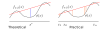
\includegraphics{../../Figures/fig_supcost.png}
	\end{figure}	
\end{frame}

\begin{frame}{$L^2$ Cost Function}
	Assume the input of the network is $x\in [0,1]$ and that the target function $\phi\colon [0,1] \to \mathbb{R}$ is square integrable. If $f_{w,b}$ is the input-output mapping, the associated cost functions measures the distance in the $L^2$ norm between the output and the target
	
	\begin{equation*}
		C(w,b)= \int_{0}^{1} (f_{w,b}(x)-\phi(x))^2 dx.
	\end{equation*}
	If the target function is known at only $n$ points
		\begin{equation*}
		z_1=\phi(x_1), z_2=\phi(x_2), \ldots, z_n= \phi(x_n)
	\end{equation*}
	then this cost function becomes the square of the Euclidean distance in $\mathbb{R}^n$ between $f_{w,b}$ and $z$
	\begin{equation*}
		C(w,b)=\sum_{i=1}^n (f_{w,b}(x_i)- z_i)^2= \| f_{w,b}(\textbf{x})-\textbf{z}\|^2
	\end{equation*}
\end{frame}

\begin{frame}{Mean Square Error Cost Function}
	Consider a neural network whose input is a random variable $X$, and its output is the random variable $Y=f_{w,b}(X)$. Assume that the network is used to approximate the target random variable $Z$. The cost function will measure the proximity between the output and the target random variables $Y$ and $Z$.  A good candidate is given by the expectation of their squared difference
	\begin{equation*}
		C(w,b)= \mathbb{E}[(Y-Z)^2]= \mathbb{E}[(f_{w,b}(X)-Z)^2]
	\end{equation*}
	Let's consider the so-called \textbf{training set} consisting of $n$ measurements of random variables $(X,Z)$, which are given by $(x_i,z_i)$. Then the cost function becomes the \textbf{empirical mean of the square difference of Y and Z}. 
	\begin{equation*}
		\hat{C}(w,b)=\frac{1}{n} \sum_{j=1}^n (f_{w,b}(x_j)- z_j)^2
	\end{equation*} 
\end{frame}

\begin{frame}{Cross-entropy}
	Let $p$ and $q$ be two densities in $\mathbb{R}$ (loosely speaking, this means that the these functions can describe a random variable).
	
	The negative likelihood function $-\ln(q(x))$ measures the information given by $q(x)$. 
	The \textbf{cross-entropy} of $p$ with respect to $q$ is defined as
	\begin{equation*}
		S(p,q)= - \int_{-\infty}^{\infty} p(x) \ln q(x) dx
	\end{equation*}
	This represents the information given by $q(x)$ assessed from the point of view of the distribution $p(x)$.
	The \textbf{Shannon entropy} is defined by 
	\begin{equation*}
		H(p)= - \int_{-\infty}^{\infty} p(x) \ln p(x) dx
	\end{equation*}
\end{frame}

\begin{frame}{Kullback-Leibler Divergence}
	The difference between the cross entropy and the Shannon entropy is the \textbf{Kullback-Leibler divergence}
	\begin{equation*}
		D_{KL}(p,q)= S(p,q)- H(p)= \int_{-\infty}^{\infty} p(x) \ln \frac{q(x)}{p(x)} dx
	\end{equation*}

	Note that KL-divergence is not a distance, but both cross-entropy and KL-divergence can be used as cost functions for neural networks.
\end{frame}

\begin{frame}{References}
	Materials and some of the pictures are from \citep{calin}.
	\printbibliography 	
	
	I have used some of the graphs by hacking TiKz code from StakExchange, Inkscape for more aesthetic plots and other old tricks of \TeX
	
\end{frame}


\end{document}
